\chapter{TỔNG QUAN VỀ ĐỀ TÀI}

\section{Sản xuất nấm ăn tại Việt Nam}

\subsection{Ý nghĩa và giá trị kinh tế của nấm}

Nấm ăn có ý nghĩa và giá trị kinh tế quan trọng trong ngành nông nghiệp và thực phẩm. Với sự đa dạng về loại hình và hương vị, nấm ăn không chỉ là một nguồn thực phẩm giàu chất dinh dưỡng mà còn mang lại những lợi ích kinh tế đáng kể.

\subsubsection{Giá trị về mặt kinh tế}
Nấm ăn là một nguồn thu nhập đáng kể cho nhiều nông dân và nhà nông. Việc trồng và thu hoạch nấm ăn tạo ra cơ hội kinh doanh và tiềm năng lợi nhuận cao. Nấm ăn có thể được trồng trong các nhà kính hoặc hệ thống nuôi trồng nấm, và thời gian từ khi gieo hạt đến thu hoạch ngắn hơn so với nhiều loại cây trồng khác. Điều này cho phép nông dân có thể tăng sản lượng và thu về lợi nhuận nhanh chóng.

\subsubsection{Giá trị về mặt thực phẩm}
Nấm là nguồn thực phẩm phong phú và đa dạng. Chúng có thể được sử dụng trong nhiều món ăn khác nhau, từ món chay cho đến món thịt. Nấm ăn không chỉ giàu chất dinh dưỡng mà còn mang lại hương vị đặc biệt và mùi thơm hấp dẫn, làm tăng giá trị và sự hấp dẫn của các món ăn. Điều này tạo ra một thị trường tiềm năng cho các nhà sản xuất, nhà hàng và các doanh nghiệp liên quan.

\subsubsection{Giá trị y học}
Nấm có nhiều giá trị về y tế và được coi là một nguồn thực phẩm chức năng. Nhiều loại nấm ăn có khả năng chống oxy hóa và tăng cường hệ miễn dịch. Chúng cũng được cho là có khả năng giảm nguy cơ mắc một số bệnh như bệnh tim mạch, tiểu đường và ung thư. Những lợi ích này đã tạo ra sự quan tâm và tăng cường nghiên cứu về nấm ăn trong lĩnh vực y học và dinh dưỡng.

Như vậy, nấm ăn không chỉ có ý nghĩa dinh dưỡng mà còn mang lại giá trị kinh tế đáng kể. Với khả năng trồng dễ dàng và thời gian thu hoạch nhanh, nấm ăn đang trở thành một lĩnh vực quan trọng trong ngành nông nghiệp và thực phẩm. Đồng thời, với hương vị đặc biệt và giá trị y tế tiềm năng, nấm ăn đáng được khám phá và khai thác trong các ngành công nghiệp liên quan.

\subsection{Thách thức trong sản xuất nấm truyền thống}

Trồng nấm truyền thống, tức là không sử dụng công nghệ và yêu cầu tay nghề cao, cũng đặt ra một số thách thức. Dưới đây là một số trong số chúng:

\subsubsection{Điều kiện môi trường}
Nấm là loại sinh vật nhạy cảm với các yếu tố môi trường như nhiệt độ, độ ẩm và ánh sáng. Trồng nấm truyền thống yêu cầu người trồng phải có kiến thức và kinh nghiệm trong việc điều chỉnh các yếu tố này. Điều kiện môi trường không ổn định hoặc không phù hợp có thể gây ra sự phát triển không đồng đều của nấm hoặc thậm chí gây chết nấm.

\subsubsection{Quản lý bệnh hại và sâu bệnh}
Nấm truyền thống dễ bị tấn công bởi bệnh hại và sâu bệnh. Các mầm bệnh và nấm mốc có thể gây ra sự suy giảm năng suất và chất lượng của nấm. Để kiểm soát bệnh hại và sâu bệnh một cách hiệu quả, người trồng nấm truyền thống cần phải có kiến thức về nhận biết và xử lý các tác nhân gây bệnh, ví dụ như thông qua việc lựa chọn giống nấm khỏe mạnh, quản lý sạch vùng trồng và sử dụng phương pháp kiểm soát sinh học hoặc hóa học phù hợp.

\subsubsection{Quản lý sự phát triển nấm}
Trồng nấm truyền thống yêu cầu sự quan sát và quản lý cẩn thận trong quá trình phát triển. Điều này bao gồm việc theo dõi sự phát triển của nấm, quản lý việc tưới nước và cung cấp chất dinh dưỡng cho nấm. Một sai sót nhỏ trong quá trình quản lý có thể ảnh hưởng đến sự phát triển và chất lượng của nấm.

\subsubsection{Yêu cầu tay nghề cao}
Trồng nấm truyền thống không sử dụng công nghệ đòi hỏi người trồng phải có kiến thức và kỹ năng cao để vượt qua những thách thức trên. Điều này đòi hỏi sự quan tâm và sự tận tụy trong việc học hỏi và cải thiện kỹ năng trồng nấm.

\subsection{Sự phát triển của công nghệ IOT và tự động hóa trong nông nghiệp}

Sự phát triển của công nghệ IoT (Internet of Things) và tự động hóa đã có một tác động đáng kể trong lĩnh vực nông nghiệp. Chúng đã mang đến nhiều lợi ích và tiềm năng cải thiện hiệu suất, hiệu quả và bền vững của các hoạt động nông nghiệp. Dưới đây là một số ví dụ về sự phát triển của công nghệ IoT và tự động hóa trong nông nghiệp:

\begin{itemize}
    \item Quản lý thông minh của nông trại: Công nghệ IoT cho phép thu thập dữ liệu từ các cảm biến và thiết bị được gắn kết trên nông trại. Thông qua việc phân tích dữ liệu, nông dân có thể theo dõi các yếu tố môi trường như nhiệt độ, độ ẩm, ánh sáng và chất lượng đất. Điều này giúp nông dân hiểu rõ hơn về điều kiện môi trường và điều chỉnh các hoạt động nông nghiệp như tưới nước, việc sử dụng phân bón và quản lý dịch bệnh một cách thông minh và hiệu quả hơn.
    \item Tự động hóa trong sản xuất nông nghiệp: Tự động hóa được áp dụng trong các hoạt động sản xuất nông nghiệp như thu hoạch, gieo hạt, tưới nước và phun thuốc. Các hệ thống tự động hóa giúp giảm sự phụ thuộc vào lao động và tăng năng suất. Chẳng hạn, các robot thu hoạch có thể phát hiện và thu hoạch quả một cách nhanh chóng và chính xác hơn, giảm thời gian và công sức lao động cần thiết.
    \item Quản lý chuỗi cung ứng thông minh: Công nghệ IoT cho phép theo dõi và quản lý thông tin về nguồn gốc, vận chuyển và lưu trữ các sản phẩm nông nghiệp. Điều này giúp tăng tính minh bạch và đảm bảo chất lượng của sản phẩm nông nghiệp. Ví dụ, các cảm biến IoT có thể được sử dụng để theo dõi nhiệt độ và độ ẩm trong kho lưu trữ, đảm bảo rằng sản phẩm được bảo quản và vận chuyển trong điều kiện tốt nhất.
    \item Hệ thống quản lý nước thông minh: Trong nông nghiệp, việc quản lý nước một cách hiệu quả là rất quan trọng. Công nghệ IoT có thể được sử dụng để giám sát và điều chỉnh việc sử dụng nước dựa trên các yếu tố như nhu cầu cây trồng, dự báo thời tiết và tình trạng đất. Hệ thống tự động tưới nước có thể điều chỉnh lượng nước được cung cấp cho cây trồng một cách chính xác, giúp tiết kiệm nước và tăng năng suất.
\end{itemize}

Như vậy, sự phát triển của công nghệ IoT và tự động hóa đã mang lại nhiều cơ hội và lợi ích trong lĩnh vực nông nghiệp. Chúng giúp nâng cao hiệu suất, tăng cường quản lý và tối thiểu công sức lao động, giảm lãng phí và tối ưu hóa quá trình sản xuất nông nghiệp. Tuy nhiên, việc triển khai công nghệ này cũng đòi hỏi đầu tư về hạ tầng và đào tạo nguồn nhân lực phù hợp để tận dụng hết tiềm năng của nó.

\section{Đặc điểm yêu cầu của hệ thống theo dõi và chăm sóc nấm}

\begin{figure}
    \centering
    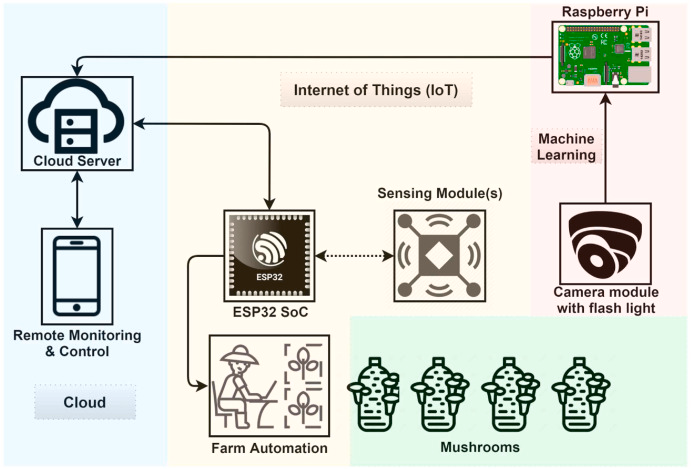
\includegraphics[width=0.5\linewidth]{images/system-example.png}
    \caption{Hệ thống mẫu trong theo dõi và chăm sóc nấm \cite{RAHMAN2022100267}}
    \label{fig:system-example}
\end{figure}

\subsection{Giám sát môi trường}

Việc trồng nấm ăn yêu cầu môi trường đặc biệt và ổn định để có thể sinh trưởng và phát triển. Vì vậy, các thiết bị giám sát môi trường trong hệ thống theo dõi và chăm sóc nấm cần đáp ứng một số đặc điểm và yêu cầu cơ bản để thu thập dữ liệu môi trường một cách chính xác và đáng tin cậy.

\subsubsection{Độ chính xác}
Thiết bị cần có độ chính xác cao trong việc đo lường các thông số môi trường như nhiệt độ, độ ẩm, ánh sáng và các thông số khác. Điều này đảm bảo rằng dữ liệu thu thập được là đáng tin cậy và chính xác để phân tích và đưa ra quyết định.
\subsubsection{Độ phủ}
Thiết bị giám sát môi trường cần có khả năng đo lường và giám sát một phạm vi rộng của môi trường nấm. Ví dụ, trong trường hợp của nấm, cần đo lường nhiệt độ và độ ẩm của không khí, độ ẩm và chất lượng đất, cường độ ánh sáng và các yếu tố khác có thể ảnh hưởng đến sự phát triển và sinh trưởng của nấm.
\subsubsection{Khả năng kết nối}
Thiết bị cần có khả năng giao tiếp và kết nối chia sẻ thông tin với hệ thống giám sát trung tâm để có thể phân tích dữ liệu và đưa ra quyết định tự động tương ứng.
\subsubsection{Hoạt động trong môi trường khắc nghiệt}
Thiết bị cần được thiết kế để chịu được điều kiện môi trường khắc nghiệt trong môi trường nấm. Nó cần có khả năng chống thời tiết, chống bụi, chống ẩm và chịu được nhiệt độ và độ ẩm biến đổi.

\subsection{Điều khiển và tự động hóa}
Trong trồng và chăm sóc nấm, điều khiển và tự động hóa có thể áp dụng để giám sát và điều chỉnh môi trường, tưới nước, chiếu sáng và các hoạt động khác đối với nấm:

\subsubsection{Điều khiển môi trường}

Hệ thống có thể được lập trình để tự động điều chỉnh nhiệt độ, độ ẩm và cường độ ánh sáng trong môi trường nấm. Cảm biến đo lường các thông số này và truyền dữ liệu đến hệ thống điều khiển, từ đó hệ thống điều khiển sẽ thực hiện các điều chỉnh cần thiết để tạo ra môi trường lý tưởng cho sự phát triển của nấm. Ví dụ, nếu nhiệt độ quá cao, hệ thống có thể kích hoạt hệ thống làm mát để giảm nhiệt độ.

Hệ thống tưới nước tự động có thể được sử dụng để cung cấp lượng nước cần thiết cho nấm một cách tự động và chính xác. Cảm biến đo lường độ ẩm đất và truyền dữ liệu đến hệ thống điều khiển. Hệ thống điều khiển có thể tự động kích hoạt hệ thống tưới nước để cung cấp nước khi độ ẩm đất thấp, và ngược lại, ngừng tưới nước khi độ ẩm đạt mức đủ.

Nấm có yêu cầu về ánh sáng để phát triển. Hệ thống điều khiển và tự động hóa có thể được sử dụng để điều chỉnh cường độ và thời gian chiếu sáng. Ví dụ, hệ thống có thể kích hoạt đèn chiếu sáng tự động để cung cấp ánh sáng cho nấm trong các khoảng thời gian nhất định hoặc điều chỉnh cường độ ánh sáng theo yêu cầu của nấm.

\subsubsection{Tự động hóa quy trình}
Hệ thống điều khiển và tự động hóa cũng có thể được sử dụng để tự động hóa các quy trình trồng và chăm sóc nấm. Ví dụ, hệ thống có thể tự động kích hoạt quy trình lấy mẫu nấm, kiểm tra chất lượng không khí, điều chỉnh môi trường, thu hoạch và các hoạt động khác.
    
\subsection{Hệ thống giám sát và phân tích}

Hệ thống giám sát và phân tích tập trung là một hệ thống được sử dụng để thu thập, theo dõi và phân tích dữ liệu từ nhiều nguồn khác nhau một cách tập trung và tổ chức. Nó cung cấp khả năng giám sát và phân tích thông tin từ các thiết bị, hệ thống và quy trình khác nhau trong một tổ chức hoặc môi trường cụ thể. Nhìn chung, hệ thống cần cung cấp khả năng giám sát và kiểm soát toàn diện, phân tích dữ liệu để tìm ra thôngtin hữu ích và hỗ trợ quyết định, và tăng cường khả năng quản lý và tối ưu hóa hoạt động của tổ chức.

\subsubsection{Thu thập dữ liệu}
Hệ thống thu thập dữ liệu từ nhiều nguồn khác nhau như cảm biến, thiết bị đo lường, hệ thống máy tính, máy móc và các nguồn dữ liệu khác. Dữ liệu này có thể bao gồm thông tin về nhiệt độ, độ ẩm, áp suất, lưu lượng, tình trạng thiết bị, dữ liệu về sản xuất và các thông số quan trọng khác.

\subsubsection{Truyền dẫn dữ liệu}
Dữ liệu được truyền từ các nguồn đến hệ thống giám sát và phân tích tập trung thông qua các kết nối mạng, giao thức truyền thông và giao thức liên kết dữ liệu khác nhau. Điều này có thể bao gồm mạng có dây, mạng không dây, giao thức Internet, giao thức truyền thông Modbus và nhiều giao thức khác.

\subsubsection{Lưu trữ và quản lý dữ liệu}
Dữ liệu được lưu trữ và quản lý trong hệ thống giám sát và phân tích tập trung. Hệ thống này thường có cơ sở dữ liệu hoặc hệ thống lưu trữ dữ liệu để lưu trữ và duy trì thông tin thu thập được. Dữ liệu có thể được lưu trữ trong thời gian thực và được cập nhật liên tục để cho phép quá trình giám sát và phân tích liên tục.

\subsubsection{Phân tích và xử lý dữ liệu}
Hệ thống giám sát và phân tích tập trung cung cấp các công cụ và phương pháp để phân tích và xử lý dữ liệu thu thập được. Điều này có thể bao gồm các thuật toán phân tích dữ liệu, công cụ học máy, công cụ thống kê và các phương pháp khác để tìm kiếm thông tin ý nghĩa từ dữ liệu và tạo ra báo cáo, biểu đồ và thông tin hữu ích khác.

\subsubsection{Giao diện người dùng và báo cáo}
Hệ thống giám sát và phân tích tập trung thường cung cấp giao diện người dùng để người dùng có thể truy cập và tương tác với dữ liệu và thông tin. Giao diện này có thể cung cấp các báo cáo, đồ thị, biểu đồ và thông tin trực quan khác để hiển thị dữ liệu và kết quả phân tích một cách dễ hiểu và tiện lợi.

\subsection{Khả năng tích hợp và mở rộng}
Khả năng tích hợp và mở rộng là hai yếu tố quan trọng khi xây dựng hệ thống giám sát và phân tích tập trung. Dưới đây là mô tả về hai khả năng này:

\subsubsection{Khả năng tích hợp}
Khả năng tích hợp đề cập đến khả năng kết nối và làm việc cùng nhau của các thành phần và hệ thống khác nhau. Trong hệ thống giám sát và phân tích tập trung, khả năng tích hợp cho phép các nguồn dữ liệu đa dạng từ các nguồn khác nhau, như cảm biến, thiết bị đo lường, hệ thống máy tính, và các hệ thống hỗ trợ khác, được kết nối và tích hợp vào một hệ thống duy nhất.

Việc có khả năng tích hợp cho phép dữ liệu từ các nguồn khác nhau được thu thập một cách đồng bộ và hiệu quả. Nó cũng giúp tạo ra một cái nhìn toàn diện và đồng nhất về dữ liệu và thông tin trong hệ thống giám sát và phân tích. Các giao thức và tiêu chuẩn quan trọng như MQTT, OPC-UA và RESTful API thường được sử dụng để đảm bảo tích hợp dữ liệu hiệu quả giữa các thành phần khác nhau trong hệ thống.

\subsubsection{Khả năng mở rộng}
Khả năng mở rộng đề cập đến khả năng mở rộng và mở rộng hệ thống giám sát và phân tích tập trung để đáp ứng nhu cầu tăng cường và mở rộng trong tương lai. Điều này bao gồm khả năng thêm mới các thiết bị, cảm biến, hệ thống và nguồn dữ liệu mới vào hệ thống một cách linh hoạt và dễ dàng.

Hệ thống giám sát và phân tích tập trung có thể được mở rộng theo hai hướng: mở rộng theo quy mô và mở rộng chức năng. Mở rộng theo quy mô liên quan đến việc gia tăng khả năng xử lý dữ liệu và lưu trữ để đáp ứng với số lượng nguồn dữ liệu lớn hơn và sự tăng trưởng của hệ thống. Mở rộng chức năng liên quan đến việc thêm mới các chức năng và tính năng mới vào hệ thống để đáp ứng với các yêu cầu và nhu cầu cụ thể.

Các kiến trúc và công nghệ như kiến trúc dựa trên dịch vụ (Service-Oriented Architecture - SOA), kiến trúc dựa trên microservices và sử dụng các công nghệ linh hoạt như điện toán đám mây (cloud computing) và ảo hóa (virtualization) có thể giúp tăng cường khả năng mở rộng của hệ thống giám sát và phân tích tập trung.

\subsection{Quản lý dữ liệu và bảo mật}
Quản lý dữ liệu và bảo mật là hai khía cạnh quan trọng trong hệ thống giám sát và phân tích tập trung. Quản lý dữ liệu đảm bảo tính toàn vẹn, tổ chức, và truy xuất dữ liệu hiệu quả, trong khi bảo mật đảm bảo rằng dữ liệu được bảo vệ khỏi các mối đe dọa an ninh và tuân thủ các quy định liên quan.

\subsubsection{Quản lý dữ liệu}
    
Quản lý dữ liệu trong hệ thống giám sát và phân tích tập trung bao gồm việc thu thập, lưu trữ, xử lý, và truy xuất dữ liệu một cách hiệu quả và có tổ chức. Các nguyên tắc quản lý dữ liệu bao gồm:

\begin{itemize}
    \item Thu thập dữ liệu: Hệ thống phải có khả năng thu thập dữ liệu từ các nguồn khác nhau và đảm bảo tính toàn vẹn và chính xác của dữ liệu thu thập được.
    \item Lưu trữ dữ liệu: Dữ liệu thu thập được cần được lưu trữ một cách an toàn và có tổ chức. Các cơ sở dữ liệu hoặc hệ thống lưu trữ dữ liệu phải được thiết kế để đảm bảo tính bền vững, khả năng mở rộng và khả năng sao lưu/phục hồi dữ liệu.
    \item Xử lý dữ liệu: Dữ liệu thu thập được cần được xử lý để tìm ra thông tin hữu ích và tạo ra các báo cáo, đồ thị, hoặc biểu đồ. Các phương pháp và công cụ phân tích dữ liệu, như học máy, thống kê, và khai phá dữ liệu, có thể được áp dụng để khai thác thông tin từ dữ liệu.
    \item Truy xuất dữ liệu: Hệ thống cần cung cấp khả năng truy xuất dữ liệu một cách nhanh chóng và dễ dàng. Giao diện người dùng và các công cụ truy xuất dữ liệu phải được thiết kế để người dùng có thể truy cập và tìm kiếm dữ liệu một cách thuận tiện.
\end{itemize}

\subsubsection{Bảo mật}
Bảo mật dữ liệu là một yếu tố quan trọng trong hệ thống giám sát và phân tích tập trung, đặc biệt khi xử lý các dữ liệu nhạy cảm hoặc quan trọng. Các biện pháp bảo mật dữ liệu bao gồm:
\begin{itemize}
    \item Quản lý quyền truy cập: Hệ thống nên áp dụng các cơ chế quản lý quyền truy cập để đảm bảo chỉ những người được ủy quyền mới có thể truy cập và xem dữ liệu nhạy cảm. Điều này có thể bao gồm việc sử dụng các phương thức chứng thực và ủy quyền, quản lý vai trò người dùng, và mã hóa dữ liệu.
    \item Mã hóa dữ liệu: Dữ liệu nhạy cảm có thể được mã hóa để đảm bảo rằng chỉ có người được ủy quyền mới có thể giải mã và truy cập dữ liệu. Các thuật toán mã hóa mạnh và các phương pháp quản lý khóa an toàn nên được sử dụng để bảo vệ dữ liệu.
    \item Giám sát và phát hiện xâm nhập: Hệ thống giám sát và phân tích tập trung nên có khả năng giám sát và phát hiện các hoạt động xâm nhập hoặc bất thường. Các công cụ giám sát an ninh, như hệ thống phát hinhập xâm nhập (Intrusion Detection System - IDS) và hệ thống phân tích hành vi (Behavioral Analytics), có thể được triển khai để phát hiện và cảnh báo về các hành vi đáng ngờ hoặc xâm nhập vào hệ thống.
    \item Sao lưu và phục hồi dữ liệu: Việc thực hiện sao lưu định kỳ và quy trình phục hồi dữ liệu là quan trọng để đảm bảo rằng dữ liệu quan trọng không bị mất đi trong trường hợp sự cố hoặc tấn công.
    \item Tuân thủ quy định: Hệ thống giám sát và phân tích tập trung cần tuân thủ các quy định và quyền riêng tư liên quan đến việc xử lý và bảo mật dữ liệu, chẳng hạn như Quy định chung về bảo vệ dữ liệu chung (GDPR) trong Liên minh châu Âu hoặc các quy định quốc gia tương tự.
\end{itemize}

\section{Sử dụng công nghệ IOT và tự động hóa trong chăm sóc nấm}

\subsection{Hệ thống cảm biến trong giám sát môi trường}

\subsubsection{Cảm biến DHT11 trong giám sát nhiệt độ, độ ẩm môi trường trồng nấm}

Cảm biến nhiệt độ - độ ẩm DHT11 là một cảm biến kỹ thuật số phổ biến được sử dụng để đo và ghi nhận nhiệt độ và độ ẩm trong môi trường.

Với thông số có độ chính xác vừa phải (Bảng \ref{tab:dht11-specs}), cảm biến DHT11 thường được sử dụng trong các ứng dụng như đo nhiệt độ và độ ẩm trong môi trường, giám sát thời tiết, kiểm soát môi trường nhiệt độ - độ ẩm trong nhà, và các ứng dụng liên quan đến IoT (Internet of Things) và nhà thông minh.

\begin{table}[]
\centering
\caption{Thông số kỹ thuật cảm biến DHT11}
\label{tab:dht11-specs}
\begin{tabular}{|l|l|}
\hline
\multicolumn{1}{|c|}{\textbf{Thông số kỹ thuật}} & \multicolumn{1}{c|}{\textbf{Giá trị}} \\ \hline
Phạm vi đo nhiệt độ                              & 0°C đến 50°C                          \\ \hline
Phạm vi đo độ ẩm                                 & 20\% đến 90\%                         \\ \hline
Độ chính xác nhiệt độ                            & ± 2°C                                 \\ \hline
Độ chính xác độ ẩm                               & ± 5\%                                 \\ \hline
Độ phân giải nhiệt độ                            & 0.1°C                                 \\ \hline
Độ phân giải độ ẩm                               & 1\%                                   \\ \hline
Điện áp hoạt động                                & 3.3V - 5V DC                          \\ \hline
Dòng tiêu thụ                                    & 1-2mA                                 \\ \hline
Giao tiếp                                        & Giao tiếp 1 dây, nhị phân             \\ \hline
Tốc độ truyền dữ liệu                            & Tối đa 1Hz (1 giây/lần)               \\ \hline
Kích thước                                       & 15.5mm x 12mm x 5.5mm                 \\ \hline
\end{tabular}
\end{table}

\subsubsection{Sử dụng Camera IP cho theo dõi và giám sát nấm}

Camera IP được sử dụng trong giám sát hình ảnh là một thiết bị mạng có khả năng ghi lại và truyền hình ảnh và âm thanh qua mạng IP. Nó cho phép người dùng từ xa quan sát và quản lý hình ảnh từ các vị trí khác nhau thông qua kết nối mạng.

Định dạng MJPEG (Motion JPEG) là một định dạng nén hình ảnh chuyển động sử dụng rộng rãi trong Camera IP. Nó sử dụng một chuỗi các khung hình JPEG độc lập để tạo ra video. Mỗi khung hình trong chuỗi MJPEG là một hình ảnh độc lập và không phụ thuộc vào các khung hình trước và sau đó. Điều này có nghĩa là mỗi khung hình có thể được giải nén và xem một cách độc lập.

Ưu điểm của định dạng MJPEG bao gồm:
\begin{itemize}
    \item Chất lượng hình ảnh tốt: MJPEG giữ được chất lượng hình ảnh cao trong mỗi khung hình do sử dụng nén JPEG độc lập cho từng khung hình.
    \item Khả năng xử lý đơn giản: Vì mỗi khung hình là độc lập, việc xử lý và truyền tải video MJPEG đơn giản hơn so với các định dạng video khác như H.264 hoặc MPEG.
    \item Khả năng tái sử dụng khung hình: Với MJPEG, các khung hình có thể dễ dàng được trích xuất và lưu trữ từ video, việc này hữu ích trong việc xem xét các sự kiện quan trọng hoặc tạo ảnh chụp nhanh từ video.
\end{itemize}

Tuy nhiên, định dạng MJPEG cũng có một số hạn chế:
\begin{itemize}
    \item Kích thước tập tin lớn: MJPEG có xu hướng tạo ra các tập tin video lớn hơn so với các định dạng nén video khác như H.264 hoặc MPEG, do mỗi khung hình được nén riêng lẻ.
    \item Băng thông mạng cao: Do kích thước tập tin lớn, việc truyền tải video MJPEG qua mạng yêu cầu băng thông cao hơn so với các định dạng video nén khác.
    \item Khả năng lưu trữ: Vì kích thước tập tin lớn, việc lưu trữ video MJPEG yêu cầu nhiều dung lượng lưu trữ hơn so với các định dạng video nén khác.
\end{itemize}

Với những ưu điểm như vậy, MJPEG là một định dạng phổ biến được sử dụng trong camera IP để giám sát hình ảnh. Đối với hệ thống giám sát sinh trưởng của nấm, nấm sinh trưởng trong thời gian dài nên hình ảnh thu nhận không yêu cầu liên tục. Như vậy, dữ liệu lưu trữ cũng không chiếm nhiều dung lượng do hình ảnh được lưu trữ rời rạc.

\subsection{Điều chỉnh điều kiện môi trường trồng nấm}

\subsection{Thiết bị giám sát và điều khiển trung tâm sử dụng Raspberry Pi 3}

Raspberry Pi 3 là một máy tính nhỏ gọn với khả năng xử lý mạnh mẽ và khả năng kết nối mạng tích hợp. Nó được sử dụng rộng rãi trong các dự án IoT, hệ thống nhúng và các ứng dụng máy tính nhỏ gọn. Với CPU Quad-Core và RAM 1GB, Raspberry Pi 3 có thể chạy các ứng dụng đa nhiệm và xử lý đa phương tiện.

Raspberry Pi 3 sử dụng khe cắm thẻ microSD để lưu trữ hệ điều hành và dữ liệu. Đối với nhu cầu lưu trữ lớn hơn và hiệu suất cao hơn, Raspberry Pi 3 cũng hỗ trợ kết nối các thiết bị lưu trữ ngoại vi như ổ cứng USB hoặc ổ SSD thông qua các cổng USB. Bằng cách kết nối một thiết bị lưu trữ ngoại vi, có thể mở rộng không gian lưu trữ và tận dụng tốc độ truyền dữ liệu nhanh hơn so với thẻ microSD (Bảng \ref{tab:rpi3-specs}.

\begin{table}[h]
\centering
\caption{Thông số kỹ thuật Raspberry Pi 3}
\label{tab:rpi3-specs}
\begin{tabular}{|l|l|}
\hline
\multicolumn{1}{|c|}{\textbf{Thông số kỹ thuật}} & \multicolumn{1}{c|}{\textbf{Giá trị}}                                                                           \\ \hline
CPU                                              & \begin{tabular}[c]{@{}l@{}}Broadcom BCM2837 64-bit Quad-Core ARM\\  Cortex-A53\end{tabular}                     \\ \hline
Tốc độ CPU                                       & 1.2 GHz                                                                                                         \\ \hline
RAM                                              & 1 GB LPDDR2 SDRAM                                                                                               \\ \hline
Kết nối mạng                                     & 10/100 Ethernet, Wi-Fi 802.11n, Bluetooth 4.2                                                                   \\ \hline
Giao diện                                        & \begin{tabular}[c]{@{}l@{}}4 cổng USB 2.0, HDMI, Ethernet, jack 3.5mm,\\Camera CSI, Display DSI\end{tabular}  \\ \hline
Đồ họa                                           & VideoCore IV 3D                                                                                                 \\ \hline
Lưu trữ                                          & Khe cắm thẻ microSD                                                                                             \\ \hline
Hệ điều hành hỗ trợ                              & \begin{tabular}[c]{@{}l@{}}Raspbian, Ubuntu, Windows 10 IoT Core\\  và các hệ điều hành Linux khác\end{tabular} \\ \hline
Kích thước                                       & 85mm x 56mm x 17mm                                                                                              \\ \hline
Nguồn điện                                       & 5V DC qua cổng micro USB                                                                                        \\ \hline
\end{tabular}
\end{table}

Raspberry Pi 3 cung cấp các giao diện và kết nối phổ biến để kết nối camera, thiết bị điều khiển và cảm biến. Dưới đây là một số phương pháp kết nối thông qua các giao diện của Raspberry Pi 3:

\subsubsection{Kết nối Camera}
Raspberry Pi 3 hỗ trợ kết nối camera thông qua giao diện Camera Serial Interface (CSI). Giao diện CSI có thể được sử dụng để kết nối các module camera tương thích với Raspberry Pi, cho phép bạn ghi lại hình ảnh hoặc thực hiện xử lý hình ảnh trực tiếp trên Pi.

\subsubsection{Kết nối Thiết bị điều khiển}
Raspberry Pi 3 hỗ trợ kết nối và điều khiển các thiết bị ngoại vi thông qua các giao diện như GPIO (General Purpose Input/Output). Các chân GPIO trên Raspberry Pi 3 cho phép người dùng kết nối và điều khiển các thiết bị như bàn phím, chuột, nút nhấn, LED, servo motor và nhiều thiết bị điều khiển khác.

\subsubsection{Kết nối Cảm biến}
Raspberry Pi 3 có thể kết nối với nhiều loại cảm biến thông qua các giao diện như GPIO và giao thức I2C. Giao diện GPIO cho phép bạn kết nối các cảm biến analog hoặc digital trực tiếp vào Raspberry Pi 3. Giao thức I2C cung cấp khả năng kết nối nhiều cảm biến thông qua một dây dẫn, giúp tiết kiệm chân kết nối.

Ngoài ra, Raspberry Pi 3 cũng hỗ trợ các giao diện khác như USB, SPI và UART cho phép kết nối và giao tiếp với các thiết bị ngoại vi khác như camera, mô đun giao tiếp không dây và các thiết bị khác.

\section{Ứng dụng công nghệ thị giác máy tính trong theo dõi và chăm sóc nấm}

\subsection{Lợi ích của công nghệ thị giác máy tính}

Ứng dụng thị giác máy tính trong trồng và theo dõi nấm có thể mang lại nhiều lợi ích quan trọng, bao gồm:

\begin{itemize}
    \item Phân loại và nhận dạng loại nấm: Thị giác máy tính có thể được sử dụng để phân loại và nhận dạng các loại nấm khác nhau. Bằng cách sử dụng các thuật toán nhận dạng hình ảnh và mô hình học máy, có thể xây dựng các hệ thống tự động phân loại nấm dựa trên hình ảnh. Điều này giúp cho việc xác định loại nấm trở nên nhanh chóng và chính xác hơn, giúp cho việc trồng và quản lý nấm hiệu quả hơn.
    \item Đếm và theo dõi sự phát triển của nấm: Thị giác máy tính có thể được sử dụng để đếm và theo dõi sự phát triển của nấm trong quá trình trồng. Bằng cách phân tích hình ảnh và xử lý dữ liệu, có thể xác định số lượng nấm, kích thước và tốc độ phát triển của chúng. Điều này giúp cho việc quản lý và điều chỉnh điều kiện trồng nấm một cách chính xác, đảm bảo sự phát triển và sản xuất nấm tốt nhất.
    \item Phát hiện bệnh và xác định tình trạng sức khỏe của nấm: Thị giác máy tính có thể được sử dụng để phát hiện các bệnh và xác định tình trạng sức khỏe của nấm. Bằng cách phân tích hình ảnh và so sánh với các mẫu dữ liệu đã biết, có thể phát hiện các dấu hiệu của bệnh hoặc tình trạng không tốt trong nấm. Điều này giúp cho việc phát hiện sớm các vấn đề và triển khai biện pháp can thiệp kịp thời để ngăn chặn sự lây lan và tổn thất nấm.
    \item Đánh giá chất lượng và thu hoạch: Thị giác máy tính có thể được sử dụng để đánh giá chất lượng của nấm và hỗ trợ trong quá trình thu hoạch. Bằng cách phân tích hình ảnh và áp dụng các tiêu chí chất lượng đã được định nghĩa trước, có thể đánh giá và phân loại nấm dựa trên kích thước, hình dạng, màu sắc và các đặc điểm khác. Điều này giúp cho việc tạo ra sản phẩm nấm có chất lượng cao và đáp ứng yêu cầu của thị trường.
\end{itemize}


\subsection{Mô hình CNN và vai trò của CNN trong phát hiện và phân loại ảnh}

CNN (Convolutional Neural Network) là một loại mô hình học sâu (deep learning) được sử dụng rộng rãi trong xử lý hình ảnh và thị giác máy tính. Nó được thiết kế đặc biệt để hiệu quả trong việc xử lý thông tin không gian và bao gồm các lớp tích chập (convolutional layers) và lớp gộp (pooling layers) để trích xuất các đặc trưng từ hình ảnh.

CNN có thể được sử dụng trong việc phát hiện và phân loại nấm:

\subsubsection{Phát hiện nấm}
CNN có thể được sử dụng để phát hiện sự hiện diện của nấm trong hình ảnh. Bằng cách huấn luyện mô hình CNN với các tập dữ liệu chứa hình ảnh nấm và không nấm, nó có thể học cách nhận diện các đặc trưng đặc biệt của nấm. Khi áp dụng mô hình này vào hình ảnh mới, nó có thể xác định xem có nấm xuất hiện hay không. Điều này có thể hữu ích trong việc đánh giá sự hiện diện nấm trong môi trường trồng hoặc trong các ứng dụng quan trọng như phát hiện nấm độc hại trong thực phẩm hoặc trong tự nhiên.

\subsubsection{Phân tích sự phát triển và tình trạng sức khỏe}
CNN có thể được sử dụng để phân tích sự phát triển và tình trạng sức khỏe của nấm dựa trên hình ảnh. Bằng cách huấn luyện mô hình CNN với các tập dữ liệu chứa hình ảnh của nấm ở các giai đoạn phát triển khác nhau hoặc ở các tình trạng sức khỏe khác nhau, nó có thể học cách nhận diện các đặc trưng liên quan. Khi áp dụng mô hình này vào hình ảnh mới, nó có thể đánh giá sự phát triển và tình trạng sức khỏe của nấm dựa trên các đặc trưng đã học được, giúp cho việc theo dõi và quản lý nấm trong quá trình trồng.

\subsection{Mô hình YOLO và ưu điểm của YOLO trong phát hiện vật thể}

YOLO (You Only Look Once) là một thuật toán phát hiện đối tượng có một số ưu điểm so với các phương pháp phát hiện đối tượng dựa trên CNN truyền thống. Dưới đây là một số ưu điểm của YOLO so với CNN:

\begin{itemize}
    \item Tốc độ: YOLO được biết đến với tốc độ suy đoán nhanh. Khác với các phương pháp phát hiện đối tượng dựa trên CNN truyền thống yêu cầu nhiều lần chạy qua các lớp ảnh hoặc cửa sổ trượt, YOLO thực hiện phát hiện đối tượng trong một lần chạy duy nhất. Điều này làm cho YOLO nhanh hơn đáng kể và hiệu quả hơn trong việc xử lý ảnh thời gian thực.
    \item Độ chính xác và đồng nhất: YOLO tạo ra các dự đoán đối tượng trực tiếp trên một lưới ô mà không cần phải xem xét các vùng đặc trưng. Điều này dẫn đến độ chính xác cao và sự đồng nhất trong việc phát hiện đối tượng. So với các phương pháp truyền thống, YOLO thường có khả năng phát hiện đối tượng nhỏ và đa dạng tốt hơn.
    \item Khả năng phát hiện đa đối tượng: YOLO có khả năng phát hiện và phân loại nhiều đối tượng trong một lần chạy. Nó có thể xác định và định vị các đối tượng không đối xứng trên cùng một hình ảnh một cách hiệu quả. Điều này làm cho YOLO phù hợp trong các ứng dụng yêu cầu phát hiện nhanh chóng và đồng thời của nhiều đối tượng.
    \item Kiến trúc đơn giản: YOLO có cấu trúc kiến trúc đơn giản và dễ hiểu. Nó bao gồm một mạng neural duy nhất và không yêu cầu quá trình rời rạc như làm việc với các cửa sổ trượt. Do đó, việc triển khai và huấn luyện YOLO trở nên đơn giản và tiện lợi.
\end{itemize}

\section{Tổng kết chương}

Chương 1 của báo cáo tập trung vào việc tìm hiểu về sản xuất nấm ăn tại Việt Nam và những thách thức mà ngành này đang phải đối mặt. Nấm được coi là loại thực phẩm có ý nghĩa và giá trị kinh tế quan trọng, tuy nhiên, sản xuất nấm truyền thống đang gặp phải nhiều khó khăn.

Chương cũng nêu rõ sự phát triển của công nghệ IoT (Internet of Things) và tự động hóa trong nông nghiệp, đặc biệt là trong sản xuất nấm. Các công nghệ này mang lại nhiều tiện ích và cơ hội mới cho ngành sản xuất nấm.

Để xây dựng hệ thống theo dõi và chăm sóc nấm hiệu quả, chương cung cấp các đặc điểm yêu cầu của hệ thống, bao gồm giám sát môi trường, điều khiển và tự động hóa, hệ thống giám sát và phân tích, khả năng tích hợp và mở rộng, quản lý dữ liệu và bảo mật.

Công nghệ IoT và tự động hóa được đề xuất và áp dụng trong chăm sóc nấm. Chương trình nêu rõ việc sử dụng hệ thống cảm biến để giám sát môi trường trồng nấm và điều chỉnh điều kiện môi trường. Ngoài ra, chương trình cũng giới thiệu thiết bị giám sát và điều khiển trung tâm sử dụng Raspberry Pi 3.

Cuối cùng, chương cung cấp một cái nhìn tổng quan về ứng dụng của công nghệ thị giác máy tính trong việc theo dõi và chăm sóc nấm. Các mô hình CNN (Convolutional Neural Network) và YOLO (You Only Look Once) được giới thiệu và giải thích vai trò của chúng trong phát hiện và phân loại ảnh.

Chương 1 giúp định hình nền tảng cho việc nghiên cứu và triển khai các hệ thống theo dõi và chăm sóc nấm sử dụng các công nghệ IoT, tự động hóa và thị giác máy tính.